% Document file for the documentation of the project
\documentclass{article}

\usepackage{graphics}
\usepackage{graphicx}
\usepackage[a4paper,
            top=2cm,
            bottom=3cm,
            left=3cm,
            right=2cm,
            marginparwidth=1.75cm
            ]{geometry}

\usepackage{float}
\usepackage{subcaption}
\usepackage{hyperref}
% \usepackage[backend=biber, style=numeric]{biblatex}

\title{Trabalho Prático - Introdução à Sistemas Lógicos}
\author{Marcos Daniel Souza Netto - 2022069492} 
\date{\today}

\begin{document}
\maketitle

\section{Introdução}

A atividade é dividida em duas partes: a primeira consiste em implementar um flip-flop D, e a segunda em implementar um \emph{One Time Pad (OTP)}, cujo propósito é cifrar uma mensagem utilizando uma operação de Ou-exclusivo com uma chave de cifragem. A seguir, serão apresentados questões sobre a implementação, os resultados obtidos e os testes implementados.

\section{\emph{Flip-Flop D}}
\subsection{Especificação Comportamental}

A especificação comportamental do flip-flop D consiste na declaração de um \emph{process} que é sensível à borda ascendente do sinal de clock. 
A cada borda ascendente do clock, o valor de \emph{D} é atribuído ao valor de \emph{Q} e \emph{~Q} recebe o sinal oposto de \emph{Q}. Esse comportamento é ilustrado na Figura \ref{fig:behavioral_wave}.

\begin{figure}[H]
    \centering
    \hfill
    \begin{subfigure}[c]{0.3\textwidth}
        \centering
        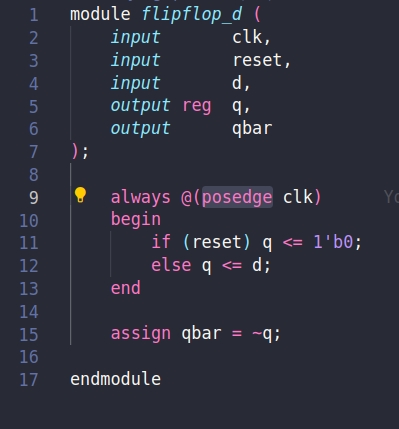
\includegraphics[width=\textwidth]{images/dflipflop_behavioral_code.png}
        \caption{Implementação em Verilog}
        \label{fig:behavioral_specification}
    \end{subfigure}
    \hfill
    \begin{subfigure}[c]{0.6\textwidth}
        \centering
        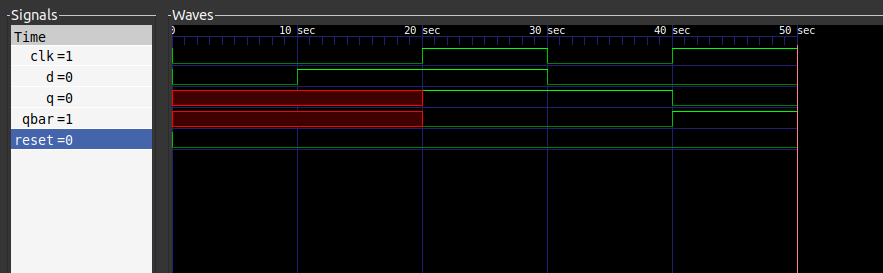
\includegraphics[width=\textwidth]{images/dflipflop_behavioral_wave.png}
        \caption{Gráfico de ondas}
        \label{fig:behavioral_wave}
    \end{subfigure}
    \hfill
    \caption{Especificação comportamental do flip-flop D}

\end{figure}

\subsection{Especificação Estrutural}
Já a especificação estrutural do flip-flop D é detalhado os componentes utilizados na construção. Dessa forma, foi definido uma \emph{Latch SR}, utilizada na contrução da \emph{Latch D}, que por sua vez é utilizada na construção do \emph{Flip-Flop D}. 
Para a construção do \emph{Flip-Flop D}, utilizamos duas \emph{Latch D}, uma como \emph{master} e outra como \emph{slave}. O comportamento do \emph{Flip-Flop D} é ilustrado na Figura \ref{fig:structural_wave}.

\begin{figure}[H]
    \centering
    \hfill
    \begin{subfigure}[c]{0.3\textwidth}
        \centering
        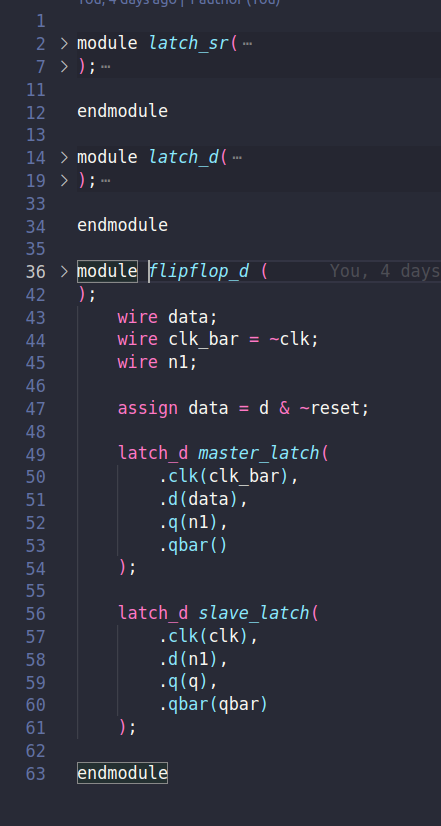
\includegraphics[width=\textwidth]{images/dflipflop_structural_code.png}
        \caption{Implementação em Verilog}
        \label{fig:structural_specification}
    \end{subfigure}
    \hfill
    \begin{subfigure}[c]{0.6\textwidth}
        \centering
        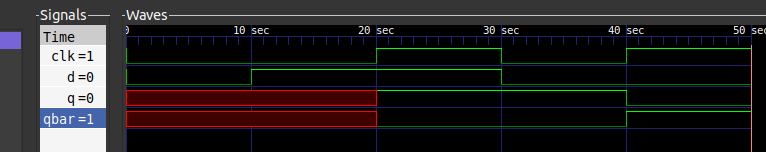
\includegraphics[width=\textwidth]{images/dflipflop_structural_wave.png}
        \caption{Gráfico de ondas}
        \label{fig:structural_wave}
    \end{subfigure}
    \hfill
    \caption{Especificação estrutural do flip-flop D}

\end{figure}

\section{Cifrador}

No cifrador implementado, temos uma mensagem de entrada (messagem a ser cifrada) e uma chave de cifragem. As messagens têm um número maior de bits do que as chaves, dessa forma, tratamos a mensagem em \emph{streams} de bits do tamanho da chave, e para cada \emph{stream} de bits, realizamos uma operação de Ou-exclusivo com a chave. Dessa forma, concatenanos os resultados dessas operações e temos a mensagem cifrada.

Para tanto, dividimos esse módulo em três submodulos: \emph{shifter},  \emph{cryptor} e \emph{cypher}.

\subsection{\emph{Shifter}}

É responsável por receber a mensagem e realizar o deslocamento da mensagem de acordo com o tamanho da chave. Dessa forma, a mensagem é dividida em \emph{streams} de bits do tamanho da chave. Que são enviados para o barramento de saída a cada borda ascendente do clock.

% Figura do shifter
\begin{figure}[H]
    \centering
    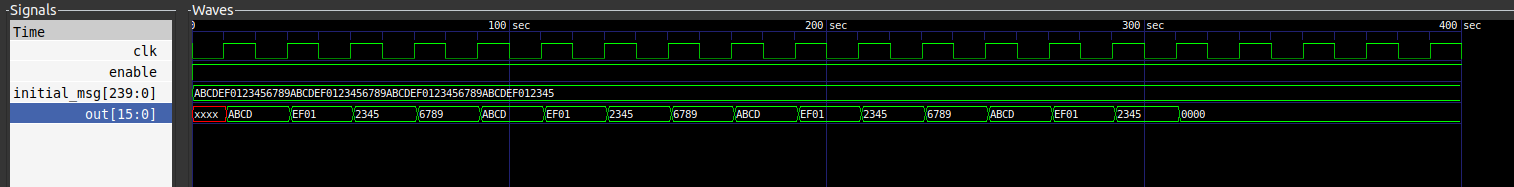
\includegraphics[width=0.95\textwidth]{images/shifter_wave.png}
    \caption{Diagrama de ondas do \emph{shifter}}
    \label{fig:shifter}
\end{figure}

\subsection{\emph{Cryptor}}
É responsável por receber a chave e realizar a operação de Ou-exclusivo com a mensagem (Ou a \emph{stream} da mensagem neste caso). Essa operação é realizada de forma contínua, ou seja, a cada modificação da mesagem ou chave, o resultado é atualizado.

\begin{figure}[H]
    \centering
    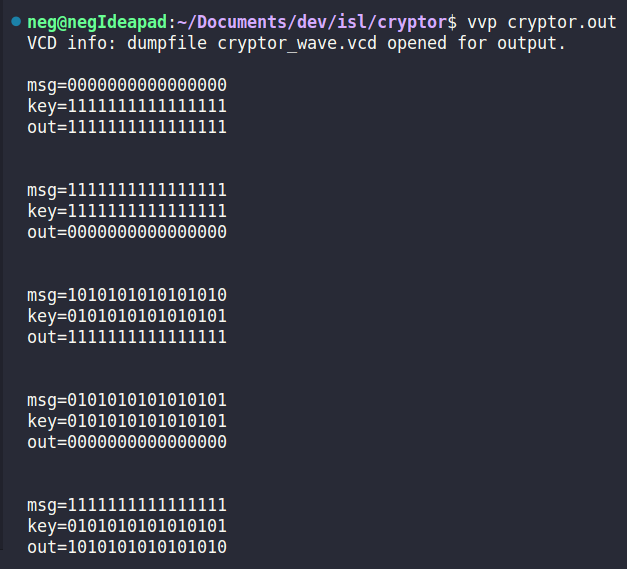
\includegraphics[width=0.6\textwidth]{images/cryptor_log.png}
    \caption{Cifragem de algumas mensagens}
    \label{fig:cryptor}
\end{figure}

\subsection{\emph{Cypher}}
É responsável por instanciar os módulos \emph{shifter} e \emph{cryptor}, e realizar a conexão entre eles. Também realiza a concatenação dos resultados do \emph{cryptor} e envia para o barramento de saída quando a mensagem está completa.

\begin{figure}[H]
    \centering
    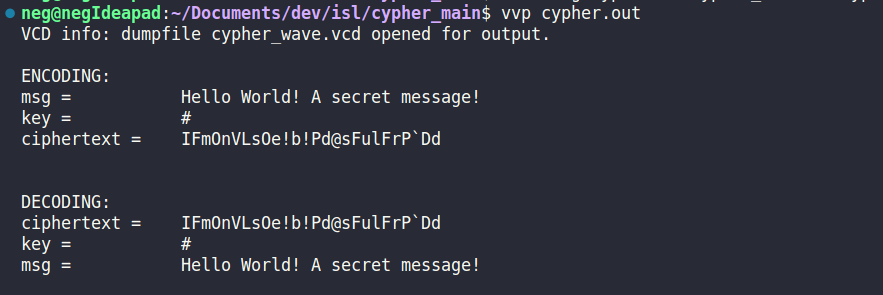
\includegraphics[width=0.9\textwidth]{images/cypher_log.png}
    \caption{Cifragem e decifragem de uma mensagem completa}
    \label{fig:cypher_log}
\end{figure}

\begin{figure}[H]
    \centering
    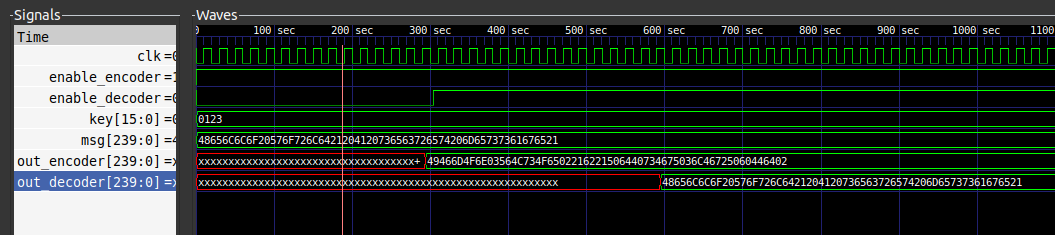
\includegraphics[width=\textwidth]{images/cypher_wave.png}
    \caption{Gráficos de ondas do \emph{cypher}}
    \label{fig:cypher_wave}
\end{figure}


\section{Testes}

Cada módulo implementado possui um arquivo de testbench, dessa forma garantimos que cada módulo está funcionando corretamente. 

Arquivos de teste:
\begin{itemize}
    \item \emph{Flip-Flop D}
        \subitem Comportamental: \emph{dflipflop\_behavioral\_tb.v} 
        \subitem Estrutural: \emph{dflipflop\_structural\_tb.v}
    \item \emph{Shifter}: \emph{shifter\_tb.v}
    \item \emph{Cryptor}: \emph{cryptor\_tb.v}
    \item \emph{Cypher}: \emph{cypher\_tb.v}
\end{itemize}

\section{Como rodar}
\subsection{EDA Playground}

Os módulos podem ser testados no \emph{EDA Playground} \footnote{\url{https://www.edaplayground.com/}}. Para isso, basta copiar o código do módulo desejado e o código do arquivo de teste correspondente, e colar no ambiente. Escolhendo o compilador \textbf{Icarus Verilog 0.9.7} e marcando a opção \textbf{Open EPWave after run}, basta clicar em rodar. 

Alternativemente, pode-se utilizar dos seguintes links para rodar os testes:
\begin{itemize}
    \item \emph{Flip-Flop D}
        \subitem Comportamental: \url{https://edaplayground.com/x/PdMx}
        \subitem Estrutural: \url{https://edaplayground.com/x/7S_N}
    \item \emph{Shifter}: \url{https://edaplayground.com/x/YkX5}
    \item \emph{Cryptor}: \url{https://edaplayground.com/x/BhA2}
    \item \emph{Cypher}: \url{https://edaplayground.com/x/ZJJT}

\end{itemize}
\subsection{Localmente}

Para rodar localmente, é necessário ter o \emph{iverilog} instalado. Após isso, basta rodar o comando: 

\begin{verbatim}
    $ iverilog <arquivo principal> <arquivo de teste> -o <nome do executavel>
\end{verbatim}
Por exemplo, para rodar o teste do \emph{Flip-Flop D} comportamental, basta rodar o comando:

\begin{verbatim}
    $ iverilog dflipflop_behavioral.sv dflipflop_behavioral_tb.v -o dflipflop_wave.out 
\end{verbatim}
    

Para executar o executável gerado, basta rodar o comando :
\begin{verbatim}
    $ vvp <nome do executavel>
\end{verbatim}

E para a visualização do gráfico de ondas, é necessário ter algum software tipo \emph{GTKWave} e assim basta rodar o comando:
\begin{verbatim}
    $ gtkwave <nome do arquivo de ondas>
\end{verbatim}


\end{document}